% \documentclass[10pt,twocolumn,letterpaper]{article}
% \usepackage{wacv}     
\documentclass[tiks]{standalone}

\usepackage{graphicx}
\usepackage{amsmath}
\usepackage{amssymb}
\usepackage{booktabs}

\usepackage{xspace}
\usepackage{svg}
\usepackage[inline]{enumitem}
\usepackage{caption}
\usepackage{subcaption}
\usepackage{makecell}
\usepackage{tikz}
\usepackage{pgfplots}

\usetikzlibrary{shapes.geometric,shapes.multipart,arrows,positioning,calc,shapes.arrows,arrows.meta,pgfplots.statistics,backgrounds,fit}
\usepgfplotslibrary{groupplots}
\tikzset{fit margins/.style={/tikz/afit/.cd,#1,
    /tikz/.cd,
    inner xsep=\pgfkeysvalueof{/tikz/afit/left}+\pgfkeysvalueof{/tikz/afit/right},
    inner ysep=\pgfkeysvalueof{/tikz/afit/top}+\pgfkeysvalueof{/tikz/afit/bottom},
    xshift=-\pgfkeysvalueof{/tikz/afit/left}+\pgfkeysvalueof{/tikz/afit/right},
    yshift=-\pgfkeysvalueof{/tikz/afit/bottom}+\pgfkeysvalueof{/tikz/afit/top}},
    afit/.cd,left/.initial=2pt,right/.initial=2pt,bottom/.initial=2pt,top/.initial=2pt}
\pgfplotsset{compat=1.18}

\newcommand{\ours}[0]{ElasticViT\xspace}
\newcommand{\dmodel}{d_{\text{model}}}
\newcommand{\afterplot}{\vspace{-.1in}} %\vspace{-.15in}}

% \newcommand{\todo}[1]{\textcolor{red}{[#1]}}
% \newcommand{\old}[1]{\textcolor{gray}{[#1]}}

% \newcommand{\janek}[2]{\textcolor{red}{#1} \textcolor{blue}{[janek: #2]}}
% \newcommand{\adam}[2]{\textcolor{red}{#1} \textcolor{blue}{[adam: #2]}}

\DeclareMathOperator{\pred}{pred}
\DeclareMathOperator{\E}{E}
\DeclareMathOperator{\miss}{miss}
\DeclareMathOperator{\scale}{scale}
\DeclareMathOperator{\pos}{pos}
\DeclareMathOperator{\PE}{PE}

\definecolor{crimson2143940}{RGB}{214,39,40}
\definecolor{darkgray176}{RGB}{176,176,176}
\definecolor{darkorange25512714}{RGB}{255,127,14}
\definecolor{forestgreen4416044}{RGB}{44,160,44}
\definecolor{gray}{RGB}{128,128,128}
\definecolor{mediumpurple148103189}{RGB}{148,103,189}
\definecolor{steelblue31119180}{RGB}{31,119,180}

\newcommand{\imsize}{1.25cm}

\begin{document}

    \begin{tikzpicture}[node distance=0.2cm, auto]
    
    \tikzstyle{header} = [text centered]
    \tikzstyle{pict} = [inner xsep=4px]
    \tikzstyle{arrow} = [thick,->,-{Latex[scale=1]}]
    

    % \node [pict, right=of input, label={[align=center]above:Edges}] (edge) {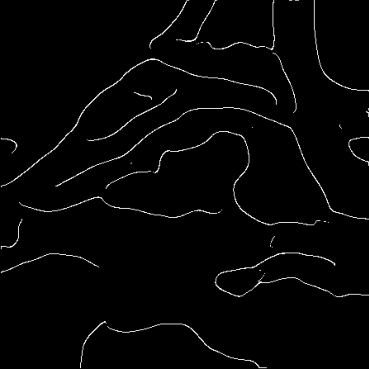
\includegraphics[width=2cm]{figures/edge/edges2.png}};
    \node [pict, label={[align=center]right:EDGE\\sampling}] (sample) {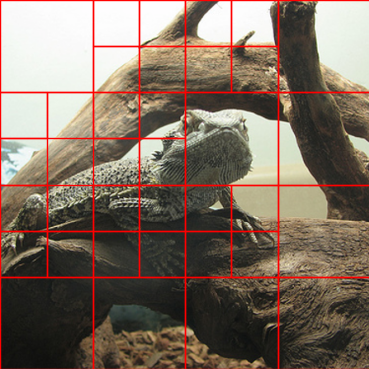
\includegraphics[width=1.8cm]{figures/edge/edges3.png}};

    \node [pict, above=of sample, label={[align=center]right:CENTRAL\\sampling}] (central) {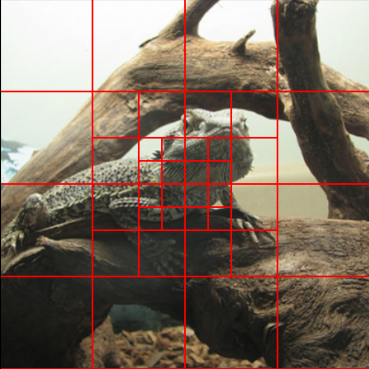
\includegraphics[width=1.8cm]{figures/edge/central.png}};


    \node[fit=(sample) (central) (central) (sample), fit margins={left=0cm,right=0cm,bottom=0cm,top=0cm}] (bbox) {};

    \node [pict, left=1cm of bbox, label={[align=center]left:Input}] (input) {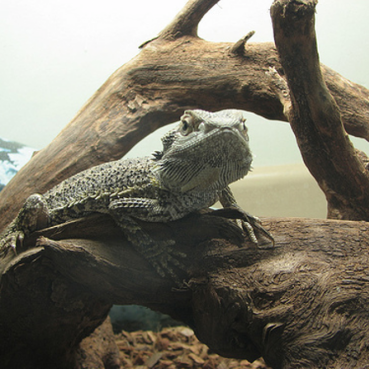
\includegraphics[width=1.8cm]{figures/edge/edges1.png}};

    \draw [arrow] (input) -- (sample);
    \draw [arrow] (input) -- (central);

    \end{tikzpicture}

\end{document}